\documentclass{beamer}
\usepackage[english,russian]{babel}
\usepackage[utf8]{inputenc}
\usepackage[usenames]{color}
\usepackage{graphicx}
\usepackage{wrapfig}
\usepackage{amsmath}
\usepackage{subfigure}
\usepackage{tikz}
\newcommand\normx[1]{\left\Vert#1\right\Vert}

% Стиль презентации
\usetheme{Warsaw}
\useoutertheme{infolines}

\newcommand\myfootnote[1]{%
  \tikz[remember picture,overlay]
  \draw (current page.south west) +(1in + \oddsidemargin,0.5em)
  node[anchor=south west,inner sep=7pt]{\parbox{\textwidth}{%
      \rlap{\rule{10em}{0.4pt}}\raggedright\scriptsize \textit{#1}}};}
    
\begin{document}
\title{On the Inductive Bias of Neural Tangent Kernels}  
\author{Nikitina Maria}
\institute{MIPT}
\date{February 18, 2025} 
% Создание заглавной страницы
\frame{\titlepage} 
%-----------------------------------------------------------------------------------------------------
\begin{frame}
    \tableofcontents
\end{frame}
%-----------------------------------------------------------------------------------------------------
\section{Motivation}
\begin{frame}
\begin{block}{Problem}
State-of-the-art neural networks are heavily over-parameterized. Optimization algorithms are crucial for learning models with good generalization properties.
\end{block}
\begin{block}{Neural tangent kernel}
In a certain overparameterized regime, the learning dynamics of gradient descent are governed by a certain kernel obtained at initialization.
\end{block}
\begin{block}{The proposal of the paper}
Studying the inductive bias of learning in such a regime by analyzing this kernel and the corresponding function space
\end{block}
\end{frame}
%-----------------------------------------------------------------------------------------------------
\section{Lazy training}
\begin{frame}
Multiple works show that when a network is sufficiently over-parameterized, weights remain close to initialization during training. The model is then well approximated by its linearization around initialization:

\[f(x, \theta) \approx f(x, \theta_0) + \langle \theta - \theta_0, \nabla_{\theta}f(x, \theta_0) \rangle.\]

This regime where weights barely move has also been referred to as \textcolor{red}{“lazy training”}[Chizat et al.].

\bigskip

\textit{Note that weak differentiability (e.g., with ReLU activations) is sufficient when studying the limiting NTK}.

\myfootnote{\href{https://arxiv.org/abs/1812.07956}{L. Chizat, E. Oyallon, and F. Bach. On lazy training in differentiable programming. NeurIPS, 2019.}}
\end{frame}
%----------------------------------------------------------------------------------------------------------
\section{Neural tangent kernels}
\begin{frame}
When the width of the network tends to infinity, the features of the linearized model tend to a limiting kernel K, called \textcolor{red}{neural tangent kernel}:

\[\langle \nabla_{\theta}f(x, \theta_0), \nabla_{\theta}f(x', \theta_0) \rangle \to K(x, x').\]

In this limit and under some assumptions, one can show that the weights move very slightly and the kernel remains fixed during training [Jacot et al.].

\bigskip

In case of finit number of model parameters convergence is allowed as long as the initial kernel matrix is non-degenerate.

\myfootnote{\href{https://arxiv.org/abs/1806.07572}{A. Jacot, F. Gabriel, and C. Hongler. Neural tangent kernel: Convergence and generalization in neural networks, NeurIPS, 2018.}}
\end{frame}
%----------------------------------------------------------------------------------------------------------
\section{NTK for two-layer ReLU networks}
\begin{frame}
Consider a two layer network of the form:

\[f(x; \theta) = \sqrt{\frac{2}{m}}\sum_{j = 1}^{m}v_j\sigma(w_j^\top x),\]

where $\sigma(u) = (u)_+ = \max(0, u)$ is the ReLU activation. The corresponding NTK is then given by:

\[K(x, x') = \|x\|\|x'\|\kappa \left(\frac{\langle x, x' \rangle}{\|x\|\|x'\|}\right),\]

where $\kappa(u) = u\kappa_0(u) + \kappa_1(u)$. $\kappa_0$ and $\kappa_1$ follow from standard calculations for arc-cosine kernels of degree $0$ and $1$.
\end{frame}
%----------------------------------------------------------------------------------------------------------
% \section{Subnetwork Inference}
% \begin{frame}
% \textbf{Lemma 1} NTK feature map for fully-connected network

% \bigskip

% The NTK for the fully-connected network can be defined as $K(x, x′) = \langle \Phi_n(x), \Phi_n(x') \rangle$, with $\Phi_0(x) = \Psi_0(x) = x$ and for $k \geq 1$:

% \[\Psi_k(x) = \varphi_1(\Psi_{k - 1}(x))\]

% \[\Phi_k(x) = \begin{pmatrix}
% \varphi_0(\Psi_{k - 1}(x)) \otimes \Phi_{k - 1}(x)\\
% \varphi_1(\Psi_{k - 1}(x))
% \end{pmatrix},\]

% where $\otimes$ is the tensor product.
% \end{frame}
%----------------------------------------------------------------------------------------------------------
\begin{frame}
\begin{block}{Smoothness}
    \begin{itemize}
        \item The kernel mapping for two-layer ReLU networks is not Lipschitz like $\kappa_1$
        \item It satisfies a weaker smoothness property similar to Hölder smoothness.
    \end{itemize}
\end{block}

\begin{block}{Approximation Properties}
    \begin{itemize}
        \item The approximation properties are studied through the spectral decomposition of the NTK. The decay rate of eigenvalues indicates how well the RKHS can approximate different types of functions.
        \item NTK for two-layer ReLU networks has better approximation properties compared to other function classes.
    \end{itemize}
\end{block}
\end{frame}
%----------------------------------------------------------------------------------------------------------
\section{NTK for CNNs}
\begin{frame}
\begin{block}{Non-linear Operator $M$}
This operator is applied point-wise to the feature maps and is essential for introducing non-linearity into the model. For two signals \( x \) and \( y \), the operator \( M \) is given by:
\[M(x, y)[u] = \begin{pmatrix}
\phi_0(x[u]) \otimes y[u] \\
\phi_1(x[u])
\end{pmatrix},\]
where $\varphi_0$ and $\varphi_1$ are kernel mappings associated with arc-cosine kernels of degrees 0 and 1, respectively.
\end{block}

\begin{block}{NTK Feature Map for CNNs}
\[\Phi(x)[u] = A_n M(x_n, y_n)[u],\]

where $A_n$ -- pooling operator.
\end{block}
\end{frame}
%----------------------------------------------------------------------------------------------------------
\begin{frame}
\begin{block}{Stability to deformation}
The NTK for CNNs provides a form of stability to deformations. The stability can be bounded, ensuring that small changes in the input lead to controlled changes in the output.
\end{block}

\begin{block}{Limitations}
Real-world CNNs with finite width may not fully exhibit the properties derived from the NTK in the infinite-width limit, leading to potential instabilities.
\end{block}

\begin{figure}
  \centering
  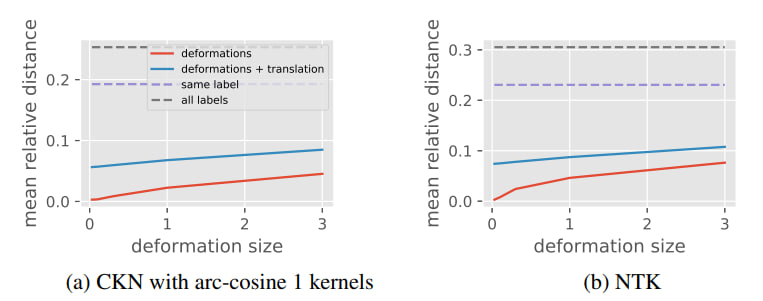
\includegraphics[width=0.75\textwidth, height=35mm]{Pictures/ntk.jpg}
\end{figure}
\end{frame}
%----------------------------------------------------------------------------------------------------------
\section{Conclusion}
\begin{frame}
\begin{enumerate}
    \item In the limit of a large number of neurons, NTK becomes constant.

    \item NTK determines how the network learns and allows analysis of function properties that can be efficiently learned.

    \item The smoothness and approximation properties of NTK help explain why over-parameterized neural networks can generalize well, even though they have many parameters.

    \item Less smooth behavior of NTK can be beneficial with large datasets.

    \item Real networks with a finite number of neurons may not fully match NTK properties.

    \item Important to balance stability and approximation when designing models.
\end{enumerate}
\end{frame}
%----------------------------------------------------------------------------------------------------------
\end{document} 